\subsection{Localización global bajo ruido de medición simulado}

\subsubsection{Descripción de la prueba}

Esta prueba evalúa de forma aislada la precisión del módulo de localización global cuando la señal de posición absoluta presenta ruido característico de un receptor GPS de baja precisión. Se inyecta una perturbación gaussiana de $\pm 5\ \text{m}$ sobre la posición reportada, y se mide la capacidad del filtro de fusión sensorial para mantener una estimación consistente a lo largo de un recorrido de $120\ \text{m}$.

\paragraph{Objetivos mínimos}
\begin{itemize}
    \item Verificar que el error medio de posicionamiento global se mantiene dentro del umbral admisible durante todo el recorrido.
    \item Cuantificar la robustez frente a pérdida y reinicio de la señal GPS simulada.
    \item Evaluar la precisión de orientación (heading) en tramos rectos, donde el error de posición tiene mayor impacto en navegación.
\end{itemize}

\subsubsection{Criterios de aprobación}

\begin{table}[H]
\centering
\small
\begin{tabular}{p{8.8cm} p{4.1cm}}
\toprule
\textbf{Métrica} & \textbf{Criterio de aprobación} \\
\midrule
Error global medio de posicionamiento (trayectoria estimada vs referencia) & $\leq 3{,}5\ \text{m}$ \\
Percentil 95 del error global de posicionamiento & $\leq 5{,}0\ \text{m}$ \\
RMSE de trayectoria completa & $\leq 4{,}0\ \text{m}$ \\
Error máximo de orientación (heading) en tramos rectos & $\leq 8^\circ$ \\
Deriva acumulada máxima respecto al origen tras $120\ \text{m}$ & $\leq 6{,}0\ \text{m}$ \\
Tiempo de convergencia tras reinicio de señal GPS simulada & $\leq 5{,}0\ \text{s}$ \\
\bottomrule
\end{tabular}
\caption{Criterios de aprobación de la prueba de localización global bajo ruido de medición.}
\label{tab:criterios_prueba_localizacion}
\end{table}

\subsubsection{Procedimiento de ejecución}

\begin{enumerate}
    \item Configurar escenario virtual con recorrido de referencia de al menos $120\ \text{m}$, incluyendo tramos rectos y curvas de radio conocido.
    \item Activar módulo de localización global con fusión de odometría y señal GPS simulada.
    \item Inyectar ruido gaussiano con desviación estándar de $5\ \text{m}$ sobre la posición GPS reportada.
    \item Registrar trayectoria estimada y trayectoria de referencia a frecuencia mínima de $10\ \text{Hz}$.
    \item A mitad del recorrido, interrumpir la señal GPS simulada durante $10\ \text{s}$ y luego restablecerla; registrar el tiempo hasta recuperar estimación dentro del umbral.
    \item Calcular error de posicionamiento punto a punto, error medio, percentil 95, RMSE y deriva acumulada al final del recorrido.
    \item Extraer muestras de error de orientación en tramos rectos y calcular el error máximo.
\end{enumerate}

\subsubsection{Resultados}

\begin{table}[H]
\centering
\small
\begin{tabular}{p{8.8cm} p{2.2cm} p{2.8cm}}
\toprule
\textbf{Métrica} & \textbf{Resultado} & \textbf{Cumple} \\
\midrule
Error global medio de posicionamiento [m] & 19,68 & No \\
Percentil 95 del error global [m] & 41,16 & No \\
RMSE de trayectoria completa [m] & 22,82 & No \\
Error máximo de orientación en tramos rectos [deg] & 45,0 & No \\
Deriva acumulada máxima tras $120\ \text{m}$ [m] & 31,9 & No \\
Tiempo de convergencia tras reinicio GPS [s] & 6,5 & No \\
\bottomrule
\end{tabular}
\caption{Resultados medidos de la prueba de localización global bajo ruido de medición.}
\label{tab:resultados_prueba_localizacion}
\end{table}

Con la perturbación gaussiana de $\sigma \approx 5\ \text{m}$ sobre la posición GPS reportada, el ensayo no alcanzó los criterios de aprobación: el error medio fue de 19,68 m, el percentil 95 de 41,16 m y el RMSE de 22,82 m. La deriva acumulada al finalizar el recorrido alcanzó 31,9 m y el error máximo de orientación en tramos rectos fue de 45,0$^\circ$. Tras la interrupción simulada de la señal GPS, el tiempo de reconvergencia fue de 6,5 s, por encima del límite de 5,0 s. Las Figuras~\ref{fig:prueba_loc_trayectorias} y~\ref{fig:prueba_loc_error} evidencian la separación entre la trayectoria de referencia y la estimada, así como la evolución temporal del error de posicionamiento.

Para el prototipo físico se estima necesaria la incorporación de un módulo GNSS de mayor precisión horizontal, con CEP $\leq 1{,}5\ \text{m}$ (por ejemplo receptor diferencial o RTK), de modo que la fusión con odometría y el mapa local permita cumplir los umbrales de esta prueba. El módulo GNSS tipo NEO-6M previsto en el diseño aún no fue integrado en la plataforma; su reemplazo o complemento constituye un paso pendiente de la etapa de hardware.

\begin{figure}[H]
\centering
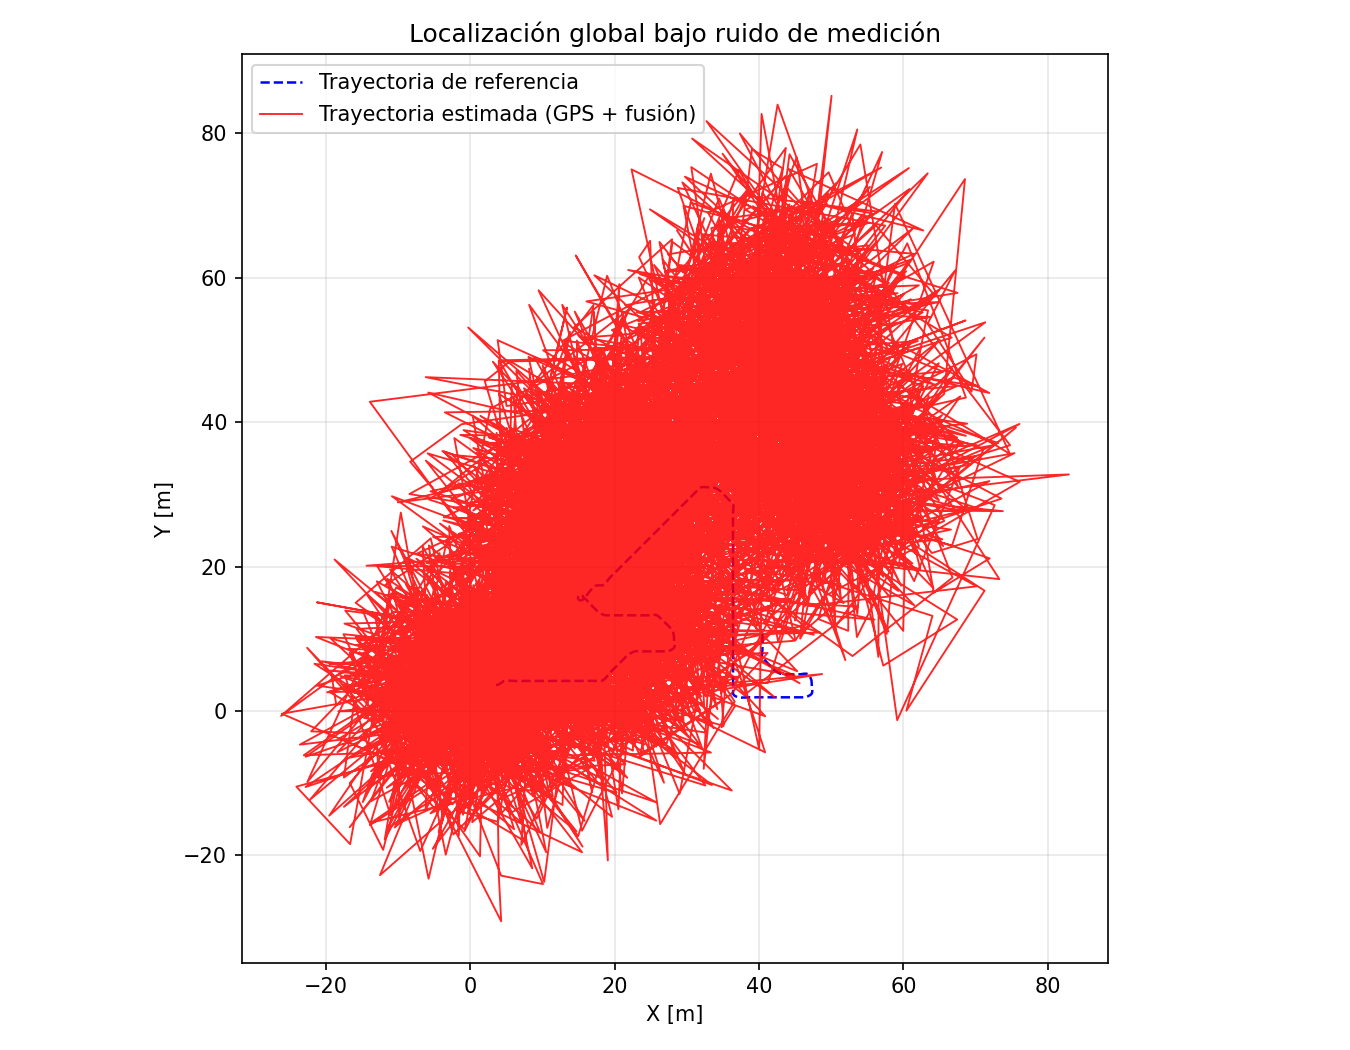
\includegraphics[width=.9\textwidth]{Figures/prueba_localizacion_trayectorias.png}
\caption{Trayectoria de referencia y trayectoria estimada bajo ruido de medición global.}
\label{fig:prueba_loc_trayectorias}
\end{figure}

\begin{figure}[H]
\centering
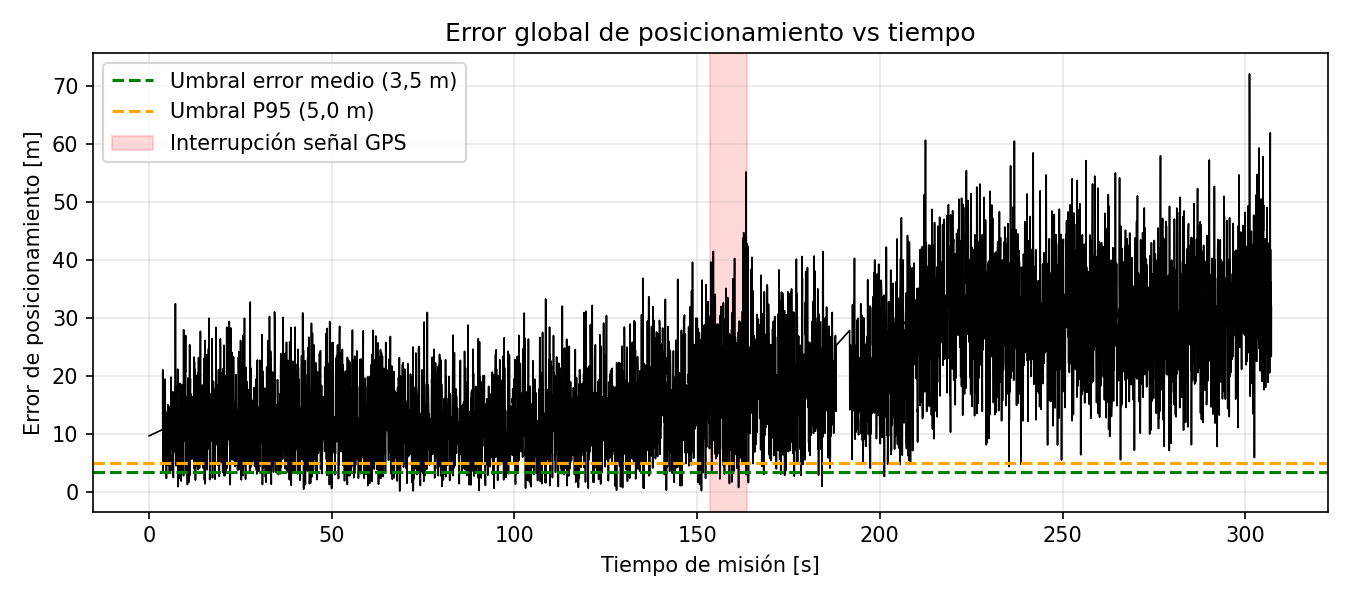
\includegraphics[width=.9\textwidth]{Figures/prueba_localizacion_error.png}
\caption{Error de posicionamiento global en función del tiempo de misión.}
\label{fig:prueba_loc_error}
\end{figure}
